\documentclass[10pt,twocolumn,letterpaper]{article}
\usepackage[T1]{fontenc}
\usepackage[pagenumbers]{cvpr}
\usepackage{amsmath,amssymb,booktabs,tabularx,multirow}
\usepackage{microtype}
\usepackage{enumitem}
\definecolor{cvprblue}{rgb}{0.21,0.49,0.74}
\usepackage[breaklinks,colorlinks,allcolors=cvprblue]{hyperref}
\hypersetup{pdftitle={OriginX: One-Shot Language Assistance under Matched Robot Replays},pdfauthor={},pdfsubject={Research manuscript}}
\def\confName{CVPR}\def\confYear{2027}
\newcommand{\policy}{\pi_{\mathrm B}}
\newcommand{\N}{1{,}004}
\newcommand{\E}{869}
\newcommand{\R}{56}
\newcommand{\F}{\mathcal F}
\newcommand{\ind}{\mathbf 1}
\newcommand{\RescuedTasks}{27}
\newcommand{\NoPilotRescues}{55}
\newcommand{\NoPilotNotRescued}{810}
\newcommand{\NoPilotUnknown}{28}
\newcommand{\NoPilotDeviation}{107}
\newcommand{\NoPilotRate}{5.50}
\newcommand{\WaitN}{869}
\newcommand{\WaitMedian}{191.38}
\newcommand{\WaitPninetyfive}{287.39}

\title{OriginX: One-Shot Language Assistance under Matched Robot Replays}
\author{Anonymous Authors}
\begin{document}
\maketitle

\begin{abstract}
Can one visual-language instruction recover a frozen robot policy's failure without additional action steps? We study all 1,004 failures from a completed 2,500-episode RoboCasa365 evaluation. Each case receives an unassisted replay and a replay with one fixed-midpoint intervention: a vision-language assistant observes three current RGB views and supplies a subgoal to the unchanged robot policy. Historical initial-state agreement, exact paired preintervention traces, and verified response application distinguish verified intervention outcomes from incomparable retries. The study verifies 56 rescues and 813 non-rescues; 28 cases remain unknown and 107 have initial-state deviations. Confirmed rescues comprise 5.58\% of the fixed cohort and 6.44\% of 869 eligible pairs. They span 27 tasks, but the five lowest-performing original tasks yield only one rescue among 237 failures. Excluding four development-exposed cases leaves 55/1,000 rescues. Median request waiting is 191 seconds, exposing an operational cost hidden by unchanged action horizons. These results characterize a limited opportunity for one-shot assistance and its replay-validity, hard-task, and latency constraints. They do not estimate a new full-benchmark score or isolate an Astra-specific reasoning advantage.
\end{abstract}

\begin{figure*}[t]
\centering
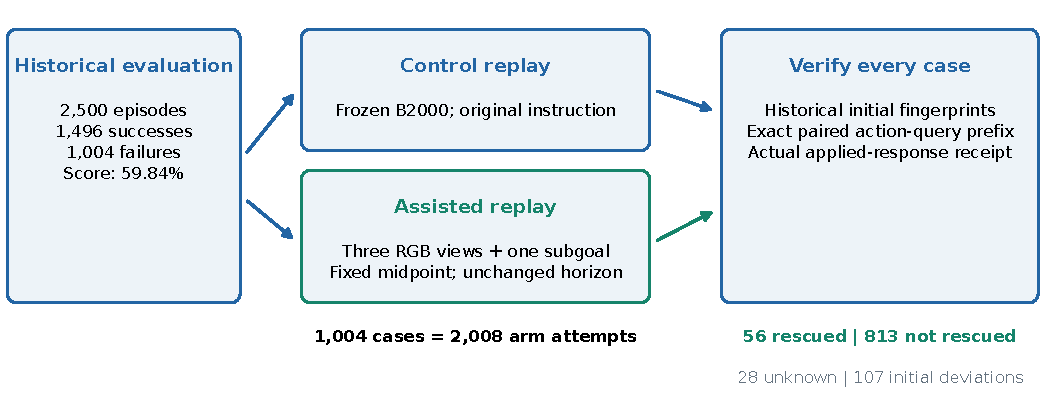
\includegraphics[width=\textwidth]{figures/protocol.pdf}
\caption{\textbf{Two records, one fixed failure cohort.} The original evaluation remains 1,496/2,500. Each of its 1,004 failures is assigned one control and one assisted replay. Assistance changes only the instruction at a fixed query; the robot weights and action horizon remain frozen. Offline replay checks and actual-response evidence determine whether the pair is eligible. All four terminal categories stay in the cohort denominator.}
\label{fig:protocol}
\end{figure*}

\section{Introduction}
\label{sec:intro}
Household manipulation couples visual interpretation with continuous control and long sequences of object interactions. Large vision-language-action (VLA) policies encode substantial behavioral knowledge, yet an instruction that is adequate at the start of a task may be insufficient after a missed grasp, an ambiguous interaction, or an unproductive continuation. Language offers an inexpensive interface in parameter space: a separate model can describe what to do next while leaving the robot policy intact. Whether that interface yields a reliable improvement is an empirical question, especially when the low-level policy was not trained to follow corrective feedback.

Prior systems use language and multimodal feedback for planning, failure explanation, and recovery~\cite{saycan,innermonologue,reflect,racer,flare}. These results motivate a narrower question: \emph{how much of a frozen policy's observed failure cohort can one image-conditioned instruction recover within its original action budget?} Answering this question requires more than showing a few successful retries. A new reset may instantiate a different scene. Two replays may have different action histories before any advice is supplied. A valid response may be generated but never reach the policy. Finally, excluding unreproducible episodes can change the population being measured.

We investigate these issues with OriginX, a frozen derivative of Xiaomi-Robotics-1-RoboCasa365~\cite{xiaomi}. A complete native-reset evaluation produces 1,496 successes and 1,004 failures across 50 tasks. We retain that evaluation as a historical record and attempt an unassisted and an assisted replay for every one of its failures. The intervention is intentionally simple: once, at the first regular policy query at or after half the horizon, an external vision-language assistant supplies a bounded next-action instruction. The robot policy continues producing motor actions. There is no new training, intervention-time simulator reset, learned failure detector, or extension of the environment-step budget.

Our emphasis is the distinction between \emph{observed assistance}, \emph{verified rescue}, and \emph{population-level improvement}. The wrapper observes only permitted images and language; privileged simulator fingerprints are used offline to verify replay comparability, never as assistant inputs. A strict rescue requires a failed control and a successful assisted replay, plus matching historical initial states, matching preintervention query traces, and linked evidence that a valid assistant response was applied. Every historical failure retains one terminal classification even if these conditions cannot be verified.

The resulting evidence is useful but bounded. We verify 56 rescues, with 813 eligible non-rescues, 28 unknowns, and 107 initial-state deviations. Recoveries occur across \RescuedTasks{} tasks, while the original Composite-Unseen split has a lower confirmed rescue fraction than either seen split. Removing the four development-exposed case identities leaves \NoPilotRescues{}/1,000 confirmed rescues. These are retrospective analyses of a fixed, failure-selected cohort; they do not establish improvement on future tasks or measure regressions on originally successful episodes.

The paper makes three contributions. First, it specifies a one-shot, observation-only assistance interface for a frozen VLA policy, with an unchanged action horizon and separately measured inference overhead. Second, it defines and executes a replay-verification procedure that distinguishes initial-state deviations, missing evidence, and valid policy outcomes without changing the fixed denominator. Third, it reports the entire 1,004-case study, including task-level heterogeneity, cost, development exposure, and unsuccessful cases. The contribution is an empirical characterization and an auditable experimental protocol, rather than a new foundation model or an assertion that language-based recovery itself is novel.



\section{Related Work}
\label{sec:related}
\paragraph{Language, feedback, and recovery.}
SayCan grounds language-model plans in robot skill affordances~\cite{saycan}. Inner Monologue feeds environmental feedback into language planning~\cite{innermonologue}. REFLECT summarizes multimodal experience to explain and correct execution failures~\cite{reflect}; RACER studies language-assisted correction and execution~\cite{racer}; FLARE targets failure-aware recovery for long-horizon manipulation~\cite{flare}. RT-H learns language-action hierarchies with correction interfaces~\cite{rth}; CycleVLA uses progress-aware transitions and backtracking~\cite{cyclevla}; ReCoVLA learns residual recovery policies with VLM guidance~\cite{recovla}. These works establish that language-mediated recovery is a developed research direction. OriginX evaluates a deliberately restricted setting: a frozen policy, one scheduled image-conditioned instruction, no iterative assistant feedback, and the original environment-step horizon. Our comparison is with the same unassisted policy. We do not reproduce these systems or claim to outperform them.

\paragraph{Policies and parameter-efficient adaptation.}
Xiaomi-Robotics-1 provides the pretrained visual-language-action model used here~\cite{xiaomi}. Its inherited capabilities dominate the scale of the system. OriginX adds an Action LoRA adapter~\cite{lora} and a small observation-conditioned modulation of the action transformer's adaptive-normalization interface, related to conditional transformer generation~\cite{dit}. Its flow-based action objective follows the released policy rather than introducing a new flow formulation~\cite{flow}. The later assistance study freezes all these components. We separate this policy substrate from the language wrapper because the available experiments do not isolate the contribution of the modulation branch.

\paragraph{Evaluation and experimental comparability.}
RoboCasa and RoboCasa365 support large-scale simulated household manipulation~\cite{robocasa,robocasa365}. We use the documented multi-task setting with pretraining scenes and Atomic-Seen, Composite-Seen, and Composite-Unseen task splits~\cite{protocol}. SIMPLER highlights the importance of carefully specified simulation interfaces when evaluating robot policies~\cite{simpler}. LIBERO-RECOVER constructs a dedicated recovery evaluation from robot failures~\cite{liberorecover}; we do not claim the first recovery benchmark. Our concern is within-study comparability: a seed and task name are not by themselves evidence of equal initial observations or equal preintervention behavior. We retain fingerprints, paired query traces, and intervention receipts alongside terminal outcomes, allowing raw retry success to be distinguished from a verified rescue.

\section{Frozen Policy and Assistance Interface}
\label{sec:method}
\subsection{The OriginX policy substrate}
Let $\theta_0$ denote the released Xiaomi checkpoint, $\alpha$ its learned Action LoRA parameters, and $\phi$ the additional conditioning branch. The policy evaluated throughout the rescue study is $\policy=\pi_{\theta_0,\alpha,\phi}$. All parameters are frozen. The branch uses three camera summaries, the last valid post-video token, and the valid 14 coordinates from each of four state-history entries. With visual-language width $D=2560$, its input has $4D+56$ coordinates. A 256-dimensional latent produces a residual with six channels of action-model width $d=1024$:
\begin{align}
z&=\operatorname{SiLU}(W_e x+b_e),\nonumber\\
\Delta_\phi(o,s)&=\operatorname{reshape}(W_\Delta z+b_\Delta,6,d).\label{eq:branch}
\end{align}
The residual is added to the released flow-time conditioning, $\widetilde m(t,o,s)=m_{\theta_0,\alpha}(t)+\Delta_\phi(o,s)$. It modifies action generation through adaptive normalization, rather than directly editing a motor command. The 4,216,839-parameter branch was trained with a flow loss, frozen-teacher retention, and training-only stage supervision; details and provenance are in the supplement. No true stage label is available at inference.

The inherited adapter's public name A2000 denotes unchanged weights trained for 1,613 updates; B2000 denotes the branch after 2,000 updates. This naming convention does not change the training record. The branch's independent benefit remains unresolved: an earlier 600-pair development comparison with the original policy found 419 versus 413 successes, with 53 B-only and 47 original-only successes (exact McNemar $p=0.6173$). That comparison changes both the adapter and branch and uses a different protocol. It is neither an ablation nor a matched baseline for the later 2,500-episode evaluation.

\subsection{A single scheduled language intervention}
The policy replans every 16 environment steps. For horizon $H$, the assistance trigger is
\begin{equation}
\tau=16\left\lceil H/32\right\rceil.
\label{eq:trigger}
\end{equation}
This is the first regular query at or after half the horizon. The trigger depends only on the fixed action budget, not on hidden success state, retrospective failure information, or a learned stall score. The original failure list selects the \emph{study cohort}; it is not an online observation supplied to the assistant.

At $\tau$, the wrapper sends the original task instruction, current left/right/wrist RGB images (256$\times$256 each), and remaining environment steps to \texttt{gpt-6-astra} at \texttt{high} reasoning effort. Routing identifiers associate each response with its case. Hidden simulator state, success predicates, future frames, and original outcome labels are excluded. The robot policy continues receiving its ordinary proprioceptive observations; these are not additionally sent to Astra.

The response provides at most 1,500 characters of subgoal text. The wrapper preserves the original instruction, appends ``Immediate next actions:'' and that text, then appends ``Then complete the original task.'' The augmented instruction persists for subsequent policy queries. Astra receives no second observation and produces no motor actions. Its generated rationale is not a verified explanation of failure.

The broker groups at most eight independent requests into labeled image contact sheets. Each response must pass the recorded schema and identity checks. The prompt forbids tool use, and event traces are checked for tool calls. The CLI invocation records the requested model and reasoning effort; it is not an independently attested identity of service-side model weights. Batch context is a shared resource and a possible source of dependence between cases, not eight separate model invocations.

\subsection{Budget and runtime invariants}
Both arms preserve seed, task, native reset, endpoint, observation history, five Euler integration steps, replanning interval, crop ratio, and registered horizon. Simulation pauses while awaiting assistance, for at most 1,200 wall-clock seconds. This wait consumes additional inference and wall time but does not add action steps. The control is therefore \emph{action-budget matched}, not compute- or latency-matched. Read-only RNG keepalives keep the same policy socket alive without reconnecting or resetting it. Missing, invalid, or unapplied responses remain technical outcomes; completed failures are not rerun to select a better outcome.

\section{Paired Replay Design}
\label{sec:design}
\subsection{Historical record and fixed cohort}
The historical native-reset evaluation contains 50 tasks with 50 episodes each: 18 Atomic-Seen, 16 Composite-Seen, and 16 Composite-Unseen, in pretraining scenes. Environment and policy seeds are fixed in $[2090900000,2090902499]$; task horizons follow RoboCasa 1.0.1. All 2,500 planned episodes have terminal records, with zero missing or infrastructure-unknown outcomes. Every failure reaches its original horizon. The original Counter reset implementation is checked before and after each episode.

We define the rescue cohort before replay as
\begin{equation}
\F=\{i:Y_i^{\mathrm{historical}}=0\},\qquad |\F|=\N.
\end{equation}
It spans 49 tasks; CloseFridge contributes no cases because its historical 50 episodes all succeeded. Each case is assigned two arms, giving 2,008 planned arm attempts but only 1,004 unique cases. The first campaign permanently claims 36 cases; an infrastructure continuation claims the other 968. This partition is fixed at whole-case level before continuation. No later outcome is substituted for a first-partition outcome.

Four infrastructure-development cases, indices 48, 97, 249, and 345, were run separately before the main study and yielded zero pilot rescues. Their pilot outcomes are excluded, but their identities remain in the primary cohort and are explicitly development-exposed. We report a leave-these-identities-out sensitivity analysis rather than describe the full cohort as untouched test data.

\subsection{Verification gates and terminal categories}
\label{sec:gates}
For each case, the verifier checks three distinct conditions. \textbf{Initial agreement} requires both replay initial fingerprints to agree with the historical case, including the recorded scene, observation, instruction, and state evidence. \textbf{Prefix agreement} requires exact paired state/image/instruction/action-query hashes before the intervention. \textbf{Applied assistance} requires linked request, image, response, CLI, and policy-query evidence showing that a valid Astra response actually reached the assisted arm. The state checks are offline measurements; their privileged contents are never policy or assistant inputs.

Let $M_i$ indicate completed arms with matching initial and preintervention evidence. Let $A_i$ indicate verified applied assistance and $E_i=M_iA_i$. The rescue indicator is
\begin{equation}
R_i=E_i\ind[Y_i^{C}=0,\ Y_i^{A}=1].
\label{eq:rescue}
\end{equation}
Here $C$ and $A$ denote the control and assisted outcomes. A valid response with no outcome, or an assisted success without matching evidence, is not a strict rescue. An eligible pair that does not satisfy the outcome transition is a non-rescue. Confirmed initial mismatches receive their own deviation category; otherwise missing or invalid evidence remains unknown. These categories are exhaustive and mutually exclusive in the settled ledger.

The checks strengthen a within-case comparison, but do not prove simulator equivalence outside the recorded contracts. In particular, preintervention traces are compared between the two new arms; they are not reconstructed historical trajectories. The historical archive contains outcome records and initial fingerprints, not videos of the original failures. We cannot retrospectively identify the original first physical error from a hash.

\subsection{What is being estimated}
We distinguish three denominators:
\begin{equation}
\widehat r_{\F}=\frac{\sum_i R_i}{1004},\quad
\widehat r_M=\frac{\sum_i R_i}{\sum_i M_i},\quad
\widehat r_E=\frac{\sum_i R_i}{\sum_i E_i}.
\label{eq:rates}
\end{equation}
The first is the confirmed rescue fraction of the fixed historical cohort. Unknowns and deviations stay in its denominator. The other two condition on evidence availability and must be read together with coverage. The cohort was selected on historical failure, so none is the overall success rate of a deployed assistance policy. The 1,496 original successes were not retested; possible assistance-induced regressions on them are unmeasured.

We treat the main counts as a census of the specified cohort. Additional task-level and uncertainty analyses are retrospective, not preregistered tests. Task-resampling intervals describe sensitivity to the represented task mixture under their resampling assumptions; they do not transform this selected cohort into a random sample of robot deployments. Technical attrition is reported directly rather than assumed missing at random.

\section{Results}
\label{sec:results}
\subsection{Baseline performance and the opportunity set}
\begin{table}[t]
\centering\small
\begin{tabular}{@{}lrrr@{}}
\toprule
Historical split & Tasks & Successes & Rate\\
\midrule
Atomic-Seen &18&747/900&83.00\%\\
Composite-Seen &16&479/800&59.88\%\\
Composite-Unseen &16&270/800&33.75\%\\
\midrule
All tasks &50&1496/2500&59.84\%\\
\bottomrule
\end{tabular}
\caption{\textbf{Frozen historical evaluation.} This single-arm record defines the later failure cohort. It is unchanged by assisted replays. Equal trials per task make the pooled rate equal to the task mean.}
\label{tab:baseline}
\end{table}
Table~\ref{tab:baseline} records the frozen endpoint. The 49.25-point Atomic-Seen versus Composite-Unseen gap motivates studying failures, but does not diagnose their causes. Composite-Unseen supplies 530 of the 1,004 failures (52.79\%). GatherTableware, HeatKebabSandwich, and PanTransfer each fail all 50 historical episodes. These failures identify an opportunity set for investigation; they do not establish that an instruction-level correction is sufficient. We omit unmatched leaderboard comparisons because different execution stacks and unavailable paired outcomes prevent attribution of small score differences.

\subsection{Verified rescue and evidence coverage}
\begin{table}[t]
\centering\small
\begin{tabular}{@{}lrr@{}}
\toprule
Terminal category & Cases & Fraction of cohort\\
\midrule
Strict rescue &56&5.58\%\\
Eligible non-rescue &813&80.98\%\\
Technical unknown &28&2.79\%\\
Initial-state deviation &107&10.66\%\\
\midrule
Fixed cohort &1004&100.00\%\\
\bottomrule
\end{tabular}
\caption{\textbf{Complete accounting, incomplete valid coverage.} All planned attempts are terminal. Unknowns and deviations are not converted to policy failures or removed from the denominator; rounded percentages need not sum exactly.}
\label{tab:coverage}
\end{table}
Table~\ref{tab:coverage} gives the complete ledger. We obtain $M=874$ matched completed replay pairs and $E=869$ pairs with verified applied assistance. Thus $R/1004=5.58\%$, $R/M=6.41\%$, and $R/E=6.44\%$. Eligibility covers 86.55\% of the fixed cohort; 13.45\% remains outside the valid intervention comparison. Reporting only the conditional 6.44\% would hide this difference.

Among eligible pairs, the complete paired table is 56 assisted-only successes and 813 failures in both arms, with zero control-only and zero both-arm successes. The 874-pair raw matched table adds five both-failure pairs whose assistance evidence is invalid; those five remain unknown, not eligible non-rescues. Their presence illustrates why terminal success bits alone cannot establish that an intervention was tested.

The first partition yields 0 rescues, 3 non-rescues, 28 unknowns, and 5 initial deviations. The continuation yields 56, 810, 0, and 102 respectively. All 28 unknowns therefore arise in the first partition. The continuation changed infrastructure handling, including same-socket keepalives and continued dispatch after validated native-reset deviations. We retain partition membership because this operational history can affect technical coverage. The study is not an uninterrupted homogeneous execution, although its endpoint, action budget, and intervention rule are fixed.

\subsection{Where assistance succeeds and where it does not}
\begin{table*}[t]
\centering\small
\begin{tabular}{@{}lrrrrrr@{}}
\toprule
Original failure split & Fixed cases & Eligible $E$ & Rescued & Unknown & Initial deviation & Rescued/fixed cases\\
\midrule
Atomic-Seen&153&137&12&0&16&7.84\%\\
Composite-Seen&321&243&25&8&70&7.79\%\\
Composite-Unseen&530&489&19&20&21&3.58\%\\
\midrule
All&1004&869&56&28&107&5.58\%\\
\bottomrule
\end{tabular}
\caption{\textbf{Task familiarity and technical coverage.} Counts are conditioned on historical failure. The lower confirmed rescue fraction in Composite-Unseen is descriptive: the splits have different tasks and horizons, and no controlled generalization effect is identified. In particular, Composite-Seen has a much higher initial-deviation count.}
\label{tab:splits}
\end{table*}
The original split breakdown appears in Table~\ref{tab:splits}. The corresponding eligible-pair rescue fractions are 12/137 (8.76\%), 25/243 (10.29\%), and 19/489 (3.89\%). Both denominator choices show fewer verified recoveries proportionally in Composite-Unseen. However, the attrition pattern differs sharply: 70/321 Composite-Seen cases have initial-state deviations, compared with 21/530 Composite-Unseen cases. This warns against assuming uniform eligibility across splits.

Rescues occur in 27 of the 49 failure-containing tasks. BreadSelection and PrepareCoffee contribute 13 of the 56 rescues (23.21\%); the five largest rescue counts contribute 24 (42.86\%). All task rows, including zero-rescue tasks, are retained in the supplement. Equal weighting of each failure-containing task gives a 7.83\% mean rescue fraction, compared with the failure-weighted 5.58\%. These answer different questions: the latter gives more weight to tasks with more historical failures.

The most difficult original tasks remain difficult after assistance. The three tasks with zero historical successes yield only one rescue among 150 failures (one among 135 eligible pairs). The five lowest historical task scores together yield one rescue among 237 failures (one among 219 eligible pairs). Thus the positive outcomes do not remove the dominant hard-task bottleneck (Fig.~\ref{fig:tasks}). These subsets are retrospective descriptions, not independently chosen test cohorts.

Resampling whole tasks within each original split (30,000 draws, fixed seed) gives a 2.5th--97.5th percentile range of 3.59--7.95\% for the failure-weighted confirmed fraction. This is an exploratory task-mixture sensitivity range, not a confidence interval for the fixed cohort or a population treatment effect. Shared assistance batches create an additional dependence not modeled by this resampling; we therefore do not use it for a significance claim.


\begin{figure}[t]
\centering
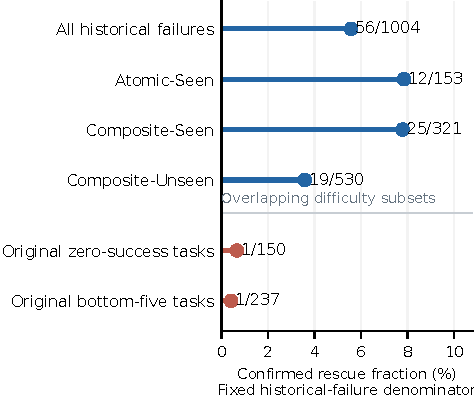
\includegraphics[width=\columnwidth]{figures/task_summary.pdf}
\caption{\textbf{Rescue heterogeneity.} Fixed-cohort rates retain technical outcomes in each denominator. The bottom two rows are overlapping subsets defined by historical task scores, not additional test cohorts. Assistance seldom resolves these difficult tasks. The supplement reports every task.}
\label{fig:tasks}
\end{figure}

\subsection{Development exposure sensitivity}
Removing all four pilot case identities leaves 1,000 historical failures with \NoPilotRescues{} rescues, \NoPilotNotRescued{} non-rescues, \NoPilotUnknown{} unknowns, and \NoPilotDeviation{} initial deviations. The confirmed fraction is \NoPilotRate{}\%, compared with 5.58\% in the full cohort. The primary results remain unchanged; this is a transparent sensitivity calculation, not a replacement test population. The pilot's separate 0/4 outcomes are never added to the primary table.

\subsection{Two matched outcomes within the same task}
\begin{figure*}[t]
\centering
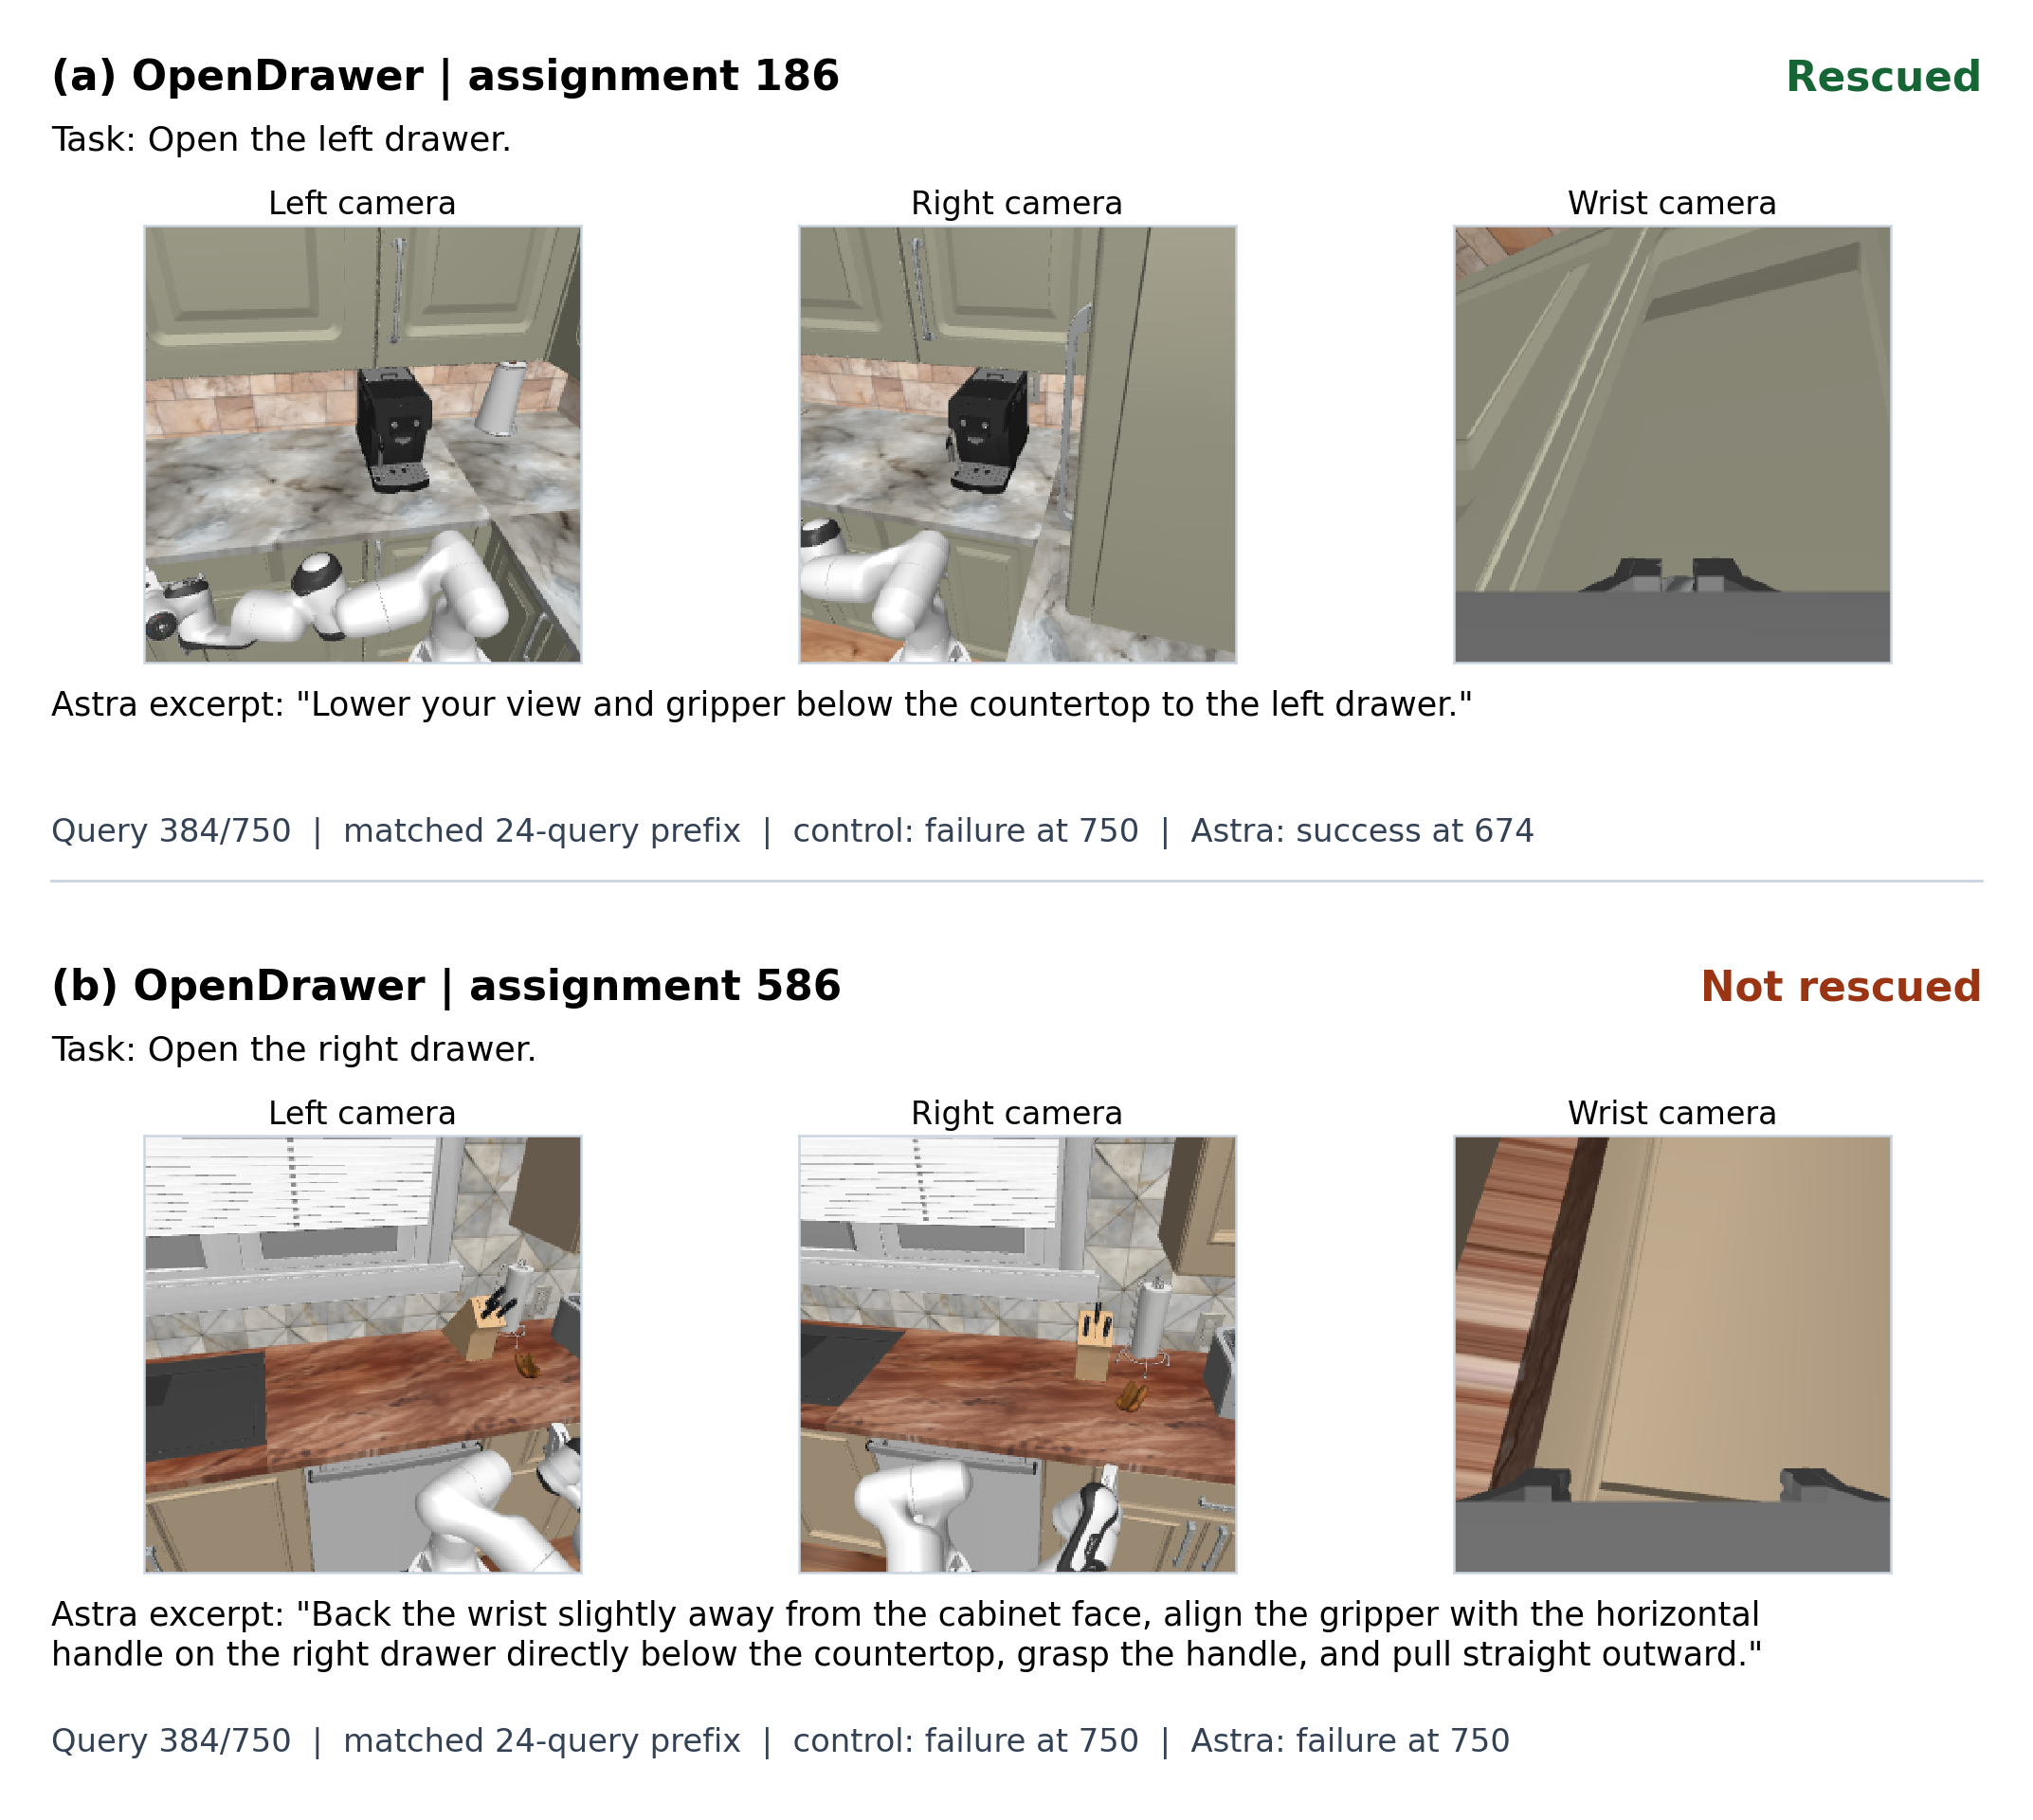
\includegraphics[width=\textwidth]{figures/cases.png}
\caption{\textbf{Actual intervention observations for both historical OpenDrawer failures.} The rows show the original three RGB views at the trigger, not reconstructed videos or generated scenes. Both pairs match their historical initial fingerprints and have 24 exact paired preintervention queries; both trigger at step 384 with horizon 750. Case 186 is rescued (assisted success at 674; control fails at 750). Case 586 is not (both fail at 750). These observations and instructions illustrate two outcomes of the same assistance interface; they do not establish a physical causal explanation.}
\label{fig:cases}
\end{figure*}
Figure~\ref{fig:cases} shows the complete two-case historical OpenDrawer failure subset. In case 186 (seed 2090900186), Astra supplies a subgoal about approaching the visible drawer handle, grasping it, and pulling outward. The applied response is linked to the policy's changed instruction. Its assisted arm succeeds at step 674, while the unassisted control exhausts the 750-step horizon. Case 586 (seed 2090900586) also receives valid advice but neither arm succeeds. Equal initial and paired-prefix evidence localizes the experimental difference to the intervention period under the checked contracts. It does not tell us which phrase, visual interpretation, or subsequent physical motion produced the positive outcome; the recorded trigger images are not a postintervention trajectory.

\subsection{Inference usage and operational latency}
\begin{table}[t]
\centering\small
\begin{tabular}{@{}lr@{}}
\toprule
Primary-study accounting & Recorded value\\
\midrule
Unique CLI invocations &135 (134 successful)\\
Known input tokens &2,592,713\\
Known output tokens &195,237\\
Reported reasoning tokens &75,511\\
Median CLI time / invocation &46.16 s\\
Median applied-request wait &\WaitMedian{} s\\
95th percentile applied-request wait &\WaitPninetyfive{} s\\
\bottomrule
\end{tabular}
\caption{\textbf{Actual inference overhead.} Invocations are deduplicated across batches and receipts. One error lacks counters; complete token totals and dollar cost are unknown. Reasoning tokens are not added again to output tokens. Request waiting includes queue/transport time and is distinct from CLI runtime.}
\label{tab:cost}
\end{table}
Table~\ref{tab:cost} separates model-service time from the robot's intervention wait. The known primary invocation latency sums to 6,186.44 seconds, with median 46.16 seconds and range 2.33--77.35 seconds. Batching means neither the sum nor the median is a per-case latency. Recorded applied-request waiting is available for \WaitN{} cases, with median \WaitMedian{} seconds and 95th percentile \WaitPninetyfive{} seconds. The successful OpenDrawer case waits 327.17 seconds even though its batch's CLI time is 48.98 seconds. This difference matters for deployment: unchanged action steps do not imply low-latency recovery.

The separate pilot uses one additional invocation with 19,071 input and 629 output tokens (137 reported reasoning tokens) and 24.35 seconds of CLI time. Failed or unapplied responses are retained in usage, so cost is not restricted to successful rescues. The authenticated CLI quota does not expose a verified monetary bill for this experiment; we do not assume zero cost or infer a price from unrelated APIs.

\section{Interpretation and Limitations}
\label{sec:limits}
\paragraph{A bounded positive finding.}
One scheduled instruction can change the outcome of some failures without weight updates or extra action steps. The verified paired evidence supports 56 such transitions in this specified cohort. At the same time, 813 eligible pairs remain unsuccessful. A larger model's textual advice is therefore not a substitute for a demonstrated control capability, and this study does not show that difficult long-horizon failures are primarily planning failures.

\paragraph{Attribution to the interface, not a unique reasoning mechanism.}
The experimental contrast changes the instruction and adds external inference. It lacks instruction-restatement, fixed generic recovery text, same-budget language-model, and multiple stochastic retries under comparable extra compute. Consequently, it cannot distinguish Astra-specific reasoning from other benefits of extra language conditioning. Nor does it identify the contribution of OriginX's continuous branch. The earlier unsuccessful paired confirmation and absent A-only ablations remain part of the evidence, not objections that can be resolved by a stronger aggregate claim.

\paragraph{Selected cases and replay attrition.}
The cohort is postselected on historical failure. Successes were not revisited, four case identities were used during infrastructure development, and unmatched or invalid pairs comprise 13.45\% of the cohort. Assistance cannot be declared beneficial overall without evaluating a frozen rule on a fresh complete manifest, including episodes it might harm. Exact recorded prefixes help isolate the within-pair intervention period but do not remove selection, possible batch dependence, simulator limitations, or service-version drift. A blinded independent rerun is still needed.

\paragraph{Reproducibility and scope.}
The evidence includes model/configuration identities, case manifests, per-arm outcomes, trace hashes, actual requests/responses, source snapshots, and deduplicated usage. The simulator uses OSMesa with disclosed rendering and context-management changes; query-pixel checks support internal consistency, not universal simulator equivalence. The release's portable loader has CPU contract checks but has not undergone a new real-model GPU parity run. These results cover one policy, one benchmark setting, and one assistance budget. They do not establish real-robot safety, cross-embodiment transfer, or SIMPLER performance. The supplement separates tested contracts from untested portability claims.

\section{Future Directions}
\label{sec:future}
\paragraph{Separate visual reasoning from extra instruction.}
The first priority is a sealed, complete evaluation comparing the frozen policy, task restatement, generic recovery text, and image-conditioned assistance at the same trigger and action horizon. Additional vision-blind and alternative-assistant arms can separate visual grounding from language-model capacity. Evaluation should include originally successful behavior, report regressions and net task-level gains, and account for extra inference rather than label action-budget matching as equal compute. No arm proposed here has been run as part of this revision.

\paragraph{Allocate assistance when it can change behavior.}
The sparse hard-task rescues and long response waits motivate an observation-only trigger that predicts when intervention is useful. A future controller could request a short plan, observe its execution, and terminate or revise assistance under a fixed total token, time, and action budget. The key test is improved rescue yield per unit overhead against the fixed midpoint rule. Trigger thresholds and retry limits must be chosen on separate development episodes, without simulator success predicates or test-outcome feedback.

\paragraph{Distill verified corrections and test transfer.}
Successful interventions could supply candidate recovery data, but instruction text alone is not an action label. Future work should record and validate the resulting state-action trajectories, retain unsuccessful attempts, and test any distilled policy on newly sealed tasks or seeds. Replication with another frozen policy and an open assistant would test portability; a distinct simulator and staged real-robot trials would test embodiment and timing constraints. Physical experiments require independent contact, stop, and latency safeguards. These directions extend the present study rather than describe capabilities already demonstrated.

\section{Conclusion}
One-shot language assistance yields 56 verified rescues among 1,004 historical failures of a frozen robot policy. Matched replay, intervention provenance, and fixed-denominator reporting reveal both this opportunity and its limits: 813 eligible non-rescues, 135 unverifiable or deviating cases, sparse hard-task recovery, and substantial waiting time. These findings motivate controlled and transferable recovery studies. The original 59.84\% evaluation remains unchanged.

{\small% Metadata verified against primary author/proceedings pages on 2026-10-09.
% SayCan uses the PMLR proceedings author order and publication year.
% Xiaomi is credited to the corporate author listed by arXiv.
% Preprints are not assigned unverified conference venues.
\begin{thebibliography}{17}

\bibitem{saycan}
Brian Ichter, Anthony Brohan, Yevgen Chebotar, et~al.
Do As I Can, Not As I Say: Grounding Language in Robotic Affordances.
In \emph{Proceedings of the 6th Conference on Robot Learning}, PMLR 205, pages 287--318, 2023.
\url{https://proceedings.mlr.press/v205/ichter23a.html}.

\bibitem{innermonologue}
Wenlong Huang, Fei Xia, Ted Xiao, Harris Chan, Jacky Liang, Pete Florence, Andy Zeng, Jonathan Tompson, Igor Mordatch, Yevgen Chebotar, Pierre Sermanet, Noah Brown, Tomas Jackson, Linda Luu, Sergey Levine, Karol Hausman, and Brian Ichter.
Inner Monologue: Embodied Reasoning through Planning with Language Models.
\emph{arXiv:2207.05608}, 2022.
\url{https://arxiv.org/abs/2207.05608}.

\bibitem{reflect}
Zeyi Liu, Arpit Bahety, and Shuran Song.
REFLECT: Summarizing Robot Experiences for Failure Explanation and Correction.
In \emph{Proceedings of the 7th Conference on Robot Learning}, PMLR 229, pages 3468--3484, 2023.
\url{https://proceedings.mlr.press/v229/liu23g.html}.

\bibitem{racer}
Yinpei Dai, Jayjun Lee, Nima Fazeli, and Joyce Chai.
RACER: Rich Language-Guided Failure Recovery Policies for Imitation Learning.
\emph{arXiv:2409.14674}, 2024.
\url{https://arxiv.org/abs/2409.14674}.

\bibitem{flare}
Ganlong Zhao, Zijia Tang, Xingping Chen, Zhanghui Kuang, Ye Tian, and Guanbin Li.
FLARE: A Failure-Aware Framework for Autonomous Correction and Recovery in Visual-Language Robotic Manipulation.
In \emph{IEEE/CVF Conference on Computer Vision and Pattern Recognition}, 2026.
\url{https://arxiv.org/abs/2608.26645}.

\bibitem{xiaomi}
Xiaomi Robotics Team.
Xiaomi-Robotics-1: Scaling Vision-Language-Action Models with over 100K Hours of Real-World Trajectories.
\emph{arXiv:2607.15330}, 2026.
\url{https://arxiv.org/abs/2607.15330}.

\bibitem{lora}
Edward J. Hu, Yelong Shen, Phillip Wallis, Zeyuan Allen-Zhu, Yuanzhi Li, Shean Wang, Lu Wang, and Weizhu Chen.
LoRA: Low-Rank Adaptation of Large Language Models.
\emph{arXiv:2106.09685}, 2021.
\url{https://arxiv.org/abs/2106.09685}.

\bibitem{dit}
William Peebles and Saining Xie.
Scalable Diffusion Models with Transformers.
In \emph{IEEE/CVF International Conference on Computer Vision}, pages 4195--4205, 2023.
\url{https://arxiv.org/abs/2212.09748}.

\bibitem{flow}
Yaron Lipman, Ricky T. Q. Chen, Heli Ben-Hamu, Maximilian Nickel, and Matt Le.
Flow Matching for Generative Modeling.
In \emph{International Conference on Learning Representations}, 2023.
\url{https://openreview.net/pdf?id=PqvMRDCJT9t}.

\bibitem{robocasa}
Soroush Nasiriany, Abhiram Maddukuri, Lance Zhang, Adeet Parikh, Aaron Lo, Abhishek Joshi, Ajay Mandlekar, and Yuke Zhu.
RoboCasa: Large-Scale Simulation of Everyday Tasks for Generalist Robots.
In \emph{Robotics: Science and Systems}, 2024.
\url{https://arxiv.org/abs/2406.02523}.

\bibitem{robocasa365}
Soroush Nasiriany, Sepehr Nasiriany, Abhiram Maddukuri, and Yuke Zhu.
RoboCasa365: A Large-Scale Simulation Framework for Training and Benchmarking Generalist Robots.
In \emph{International Conference on Learning Representations}, 2026.
\url{https://robocasa.ai/}.

\bibitem{protocol}
RoboCasa Team.
Multi-Task Learning.
\emph{RoboCasa 1.0.1 Documentation}, accessed October 9, 2026.
\url{https://robocasa.ai/docs/build/html/benchmarking/multitask_learning.html}.

\bibitem{simpler}
Xuanlin Li, Kyle Hsu, Jiayuan Gu, Karl Pertsch, Oier Mees, Homer Rich Walke, Chuyuan Fu, Ishikaa Lunawat, Isabel Sieh, Sean Kirmani, Sergey Levine, Jiajun Wu, Chelsea Finn, Hao Su, Quan Vuong, and Ted Xiao.
Evaluating Real-World Robot Manipulation Policies in Simulation.
\emph{arXiv:2405.05941}, 2024.
\url{https://arxiv.org/abs/2405.05941}.

\bibitem{rth}
Suneel Belkhale, Tianli Ding, Ted Xiao, Pierre Sermanet, Quon Vuong, Jonathan Tompson, Yevgen Chebotar, Debidatta Dwibedi, and Dorsa Sadigh.
RT-H: Action Hierarchies Using Language.
\emph{arXiv:2403.01823}, 2024.
\url{https://arxiv.org/abs/2403.01823}.

\bibitem{cyclevla}
Chenyang Ma, Kai Lu, Guangyu Yang, Jiuming Liu, Shitong Xu, Bill Byrne, Ioannis Havoutis, Niki Trigoni, and Andrew Markham.
CycleVLA: Proactive Self-Correcting Vision-Language-Action Models via Subtask Backtracking and Minimum Bayes Risk Decoding.
\emph{arXiv:2601.02295}, 2026.
\url{https://arxiv.org/abs/2601.02295}.

\bibitem{recovla}
Haodi Hu, Chung-Ta Huang, Jing Liu, Ye Wang, Kei Suzuki, Matthew Brand, and Toshiaki Koike-Akino.
ReCoVLA: VLM-Guided Reward Compilation for Failure Recovery in Vision-Language-Action Policies.
\emph{arXiv:2606.09630}, 2026.
\url{https://arxiv.org/abs/2606.09630}.

\bibitem{liberorecover}
Lin Liu, Zhicheng Bao, Lu Zhang, Ziying Song, Wu Yang, Yuzheng Zhuang, Shuai Tao, Wulong Liu, Caiyan Jia, and Huchuan Lu.
LIBERO-RECOVER: Beyond Task Success Towards Failure Recovery in Robotic Manipulation Models.
\emph{arXiv:2609.05178}, 2026.
\url{https://arxiv.org/abs/2609.05178}.

\end{thebibliography}
}
\end{document}
